%************************************************************************************************************************************

\section{Experiments}
\subsection{Settings}
\noindent \textbf{Training Details:}
In general, our PU-Transformer is implemented using Tensorflow~\cite{abadi2016tensorflow} with a single GeForce 2080 Ti GPU running on the Linux OS. In terms of the hyperparameters for training, we heavily adopt the settings from PU-GCN~\cite{qian2021pu} and Dis-PU~\cite{li2021point} for the experiments in Tab.~\ref{tab:pu1k} and Tab.~\ref{tab:pugan}, respectively. For example, we have a batch size of 64 for 100 training epochs, an initial learning rate of $1\times10^{-3}$ with a 0.7 decay rate, \etc~Moreover, we only use the modified Chamfer Distance loss~\cite{yifan2019patch} to train the PU-Transformer, minimizing the average closest point distance between the input set $\mathcal{P}\in\mathbb{R}^{N\times3}$ and the output set $\mathcal{S}\in\mathbb{R}^{rN\times3}$ for efficient and effective convergence. 

\noindent \textbf{Datasets:} 
Basically, we apply two 3D benchmarks for our experiments: 
\begin{itemize}
 \item \textbf{PU1K:} 
This is a new point cloud upsampling dataset introduced in PU-GCN~\cite{qian2021pu}. In general, the PU1K dataset incorporates 1,020 3D meshes for training and 127 3D meshes for testing, where most 3D meshes are collected from ShapeNetCore~\cite{chang2015shapenet} covering 50 object categories. To fit in with the patch-based upsampling pipeline~\cite{yifan2019patch}, the training data is generated from patches of 3D meshes via Poisson disk sampling. Specifically, the training data includes 69,000 samples, where each sample has 256 input points (low resolution) and a ground-truth of 1,024 points ($4\times$ high resolution).
 \item \textbf{PU-GAN Dataset:} 
This is an earlier dataset that was first used in PU-GAN~\cite{li2019pu} and generated in a similar way as PU1K but on a smaller scale. To be concrete, the training data comprises 24,000 samples (patches) collected from 120 3D meshes, while the testing data only contains 27 meshes. In addition to the PU1K dataset consisting of a large volume of data targeting the basic $4\times$ upsampling experiment, we conduct both $4\times$ and $16\times$ upsampling experiments based on the compact data of the PU-GAN dataset.

\end{itemize}

\noindent \textbf{Evaluation Metrics:}
As for the testing process, we follow common practice that has been utilized in previous point cloud upsampling works~\cite{yifan2019patch,li2019pu,li2021point,qian2021pu}. To be specific, at first, we cut the input point cloud into multiple seed patches covering all the $N$ points. Then, we apply the trained PU-Transformer model to upsample the seed patches with a scale of $r$. Finally, the farthest point sampling algorithm~\cite{qi2017pointnet} is used to combine all the upsampled patches as a dense output point cloud with $rN$ points. For the $4\times$ upsampling experiments in this paper, each testing sample has a low-resolution point cloud with 2,048 points, as well as a high-resolution one with 8,196 points. Coupled with the original 3D meshes, we quantitatively evaluate the upsampling performance of our PU-Transformer based on three widely used metrics: (i) Chamfer Distance (CD), (ii) Hausdorff Distance~\cite{berger2013benchmark} (HD), and (iii) Point-to-Surface Distance (P2F). A lower value under these metrics denotes better upsampling performance.

%Besides, the testing data is sampled from the whole 3D meshes, where each sample has 2,048 input points and 8,096 ground-truth points.

\begin{table}
\begin{center}
\captionsetup{font=small, skip=3pt}
\caption{Quantitative comparisons ($4\times$ Upsampling) to state-of-the-art methods on the \emph{PU1K} dataset~\cite{qian2021pu}. (\enquote{\textbf{CD}}: Chamfer Distance; \enquote{\textbf{HD}}: Hausdorff Distance; \enquote{\textbf{P2F}}: Point-to-Surface Distance. \enquote{\textbf{Model}}: model size; \enquote{\textbf{Time}}: average inference time per sample; \enquote{\textbf{Param.}}: number of parameters. $^\ast$: self-reproduced results, --: unknown data.)}
\resizebox{0.6\columnwidth}{!}{
\begin{tabular}{|c|ccc|ccc|}
\Xhline{3\arrayrulewidth}
\multirow{2}{*}{Methods} &\textbf{Model} &\textbf{Time}  &\textbf{Param.} &\multicolumn{3}{c|}{Results ($\times {10}^{-3}$)}  \\\cline{5-7}
&(MB) &($\times {10}^{-3}$s)  &($\times10^3$) &\textbf{CD} $\downarrow$ &\textbf{HD} $\downarrow$ &\textbf{P2F} $\downarrow$  \\\hline\xrowht{7pt}
PU-Net~\cite{yu2018pu} &10.1 &8.4  &812.0 &1.155 &15.170 &4.834                 \\
MPU~\cite{yifan2019patch} &6.2 &8.3  &76.2 &0.935 &13.327 &3.551                 \\
PU-GACNet~\cite{han2022pu} &-- &-- &\textbf{50.7} &0.665 &9.053 &2.429 \\
PU-GCN~\cite{qian2021pu} &\textbf{1.8} &\textbf{8.0}  &76.0 &0.585 &7.577 &2.499             \\
Dis-PU$^\ast$~\cite{li2021point} &13.2 &10.8  &1047.0 &0.485 &6.145 &1.802             \\\hline
\rowcolor{Gray} \textbf{Ours} &18.4 &9.9  &969.9 &\textbf{0.451} &\textbf{3.843} &\textbf{1.277}\\\Xhline{3\arrayrulewidth}      
\end{tabular}
\label{tab:pu1k}
}
\end{center}
\end{table}

\begin{table}
\begin{center}
\captionsetup{font=small, skip=3pt}
\caption{Quantitative comparisons to state-of-the-art methods on the \emph{PU-GAN} dataset~\cite{li2019pu}. (All metric units are ${10}^{-3}$. The best results are denoted in \textbf{bold}.)}
\resizebox{0.6\columnwidth}{!}{
\begin{tabular}{|c|ccc|ccc|}
\Xhline{3\arrayrulewidth}
\multirow{2}{*}{Methods} &\multicolumn{3}{c|}{$4\times$ Upsampling} &\multicolumn{3}{c|}{$16\times$ Upsampling}  \\\cline{2-7}
&\textbf{CD} $\downarrow$ &\textbf{HD} $\downarrow$ &\textbf{P2F} $\downarrow$ &\textbf{CD} $\downarrow$ &\textbf{HD} $\downarrow$ &\textbf{P2F} $\downarrow$ \\\hline
PU-Net~\cite{yu2018pu} &0.844 &7.061 &9.431 &0.699 &8.594 &11.619               \\
MPU~\cite{yifan2019patch} &0.632 &6.998 &6.199 &0.348 &7.187 &6.822                 \\
PU-GAN~\cite{li2019pu} &0.483 &5.323 &5.053 &0.269 &7.127 &6.306             \\
PU-GCN$^\ast$~\cite{qian2021pu} &0.357 &5.229 &3.628 &0.256 &5.938 &3.945\\
Dis-PU~\cite{li2021point} &0.315 &4.201 &4.149 &\textbf{0.199} &4.716 &4.249             \\\hline
\rowcolor{Gray}\textbf{Ours} &\textbf{0.273} &\textbf{2.605} &\textbf{1.836} &0.241 &\textbf{2.310} &\textbf{1.687}    \\\Xhline{3\arrayrulewidth}      
\end{tabular}
\label{tab:pugan}
}
\end{center}
\end{table}


\subsection{Point Cloud Upsampling Results}
\label{sec:results}
\noindent \textbf{PU1K:}
Table~\ref{tab:pu1k} shows the quantitative results of our PU-Transformer on the PU1K dataset. It can be seen that our approach outperforms other state-of-the-art methods on all three metrics. In terms of the Chamfer Distance metric, we achieve the best performance among all the tested networks, since the reported values of others are all higher than ours of 0.451. Under the other two metrics, the improvements of PU-Transformer are particularly significant: compared to the performance of the recent PU-GCN~\cite{qian2021pu}, our approach can almost \emph{halve} the values assessed under both the Hausdorff Distance (HD: 7.577$\rightarrow$3.843) and the Point-to-Surface Distance (P2F: 2.499$\rightarrow$1.277). 

\noindent \textbf{PU-GAN Dataset:}
We also conduct point cloud upsampling experiments using the dataset introduced in PU-GAN~\cite{li2019pu}. under more upsampling scales. As shown in Table~\ref{tab:pugan}, we achieve best performance under all three evaluation metrics for the $4\times$ upsampling experiment. However, in the $16\times$ upsampling test, we (CD: 0.241) are slightly behind the latest Dis-PU network~\cite{li2021point} (CD: 0.199) evaluated under the Chamfer Distance metric: the Dis-PU applies two CD-related items as its loss function, hence getting an edge for CD metric only. As for the results under Hausdorff Distance and Point-to-Surface Distance metrics, our PU-Transformer shows significant improvements again, where some values (\eg, P2F in $4\times$, HD and P2F in $16\times$) are even lower than \emph{half} of Dis-PU's results.

\begin{table}
\begin{center}
\captionsetup{font=small, skip=3pt}
\caption{Ablation study of the PU-Transformer's components tested on the \emph{PU1K} dataset~\cite{qian2021pu}. Specifically, models $A_1$-$A_3$ investigate the effects of the Positional Fusion block, models $B_1$-$B_3$ compare the results of different self-attention approaches, and models $C_1$-$C_3$ test the upsampling methods in the tail.}
\resizebox{0.8\columnwidth}{!}{
\begin{tabular}{c|c|c|c|ccc}
\Xhline{3\arrayrulewidth}
\multirow{2}{*}{models} & \multicolumn{2}{c|}{PU-Transformer Body} & \multirow{2}{*}{PU-Transformer Tail} & \multicolumn{3}{c}{Results ($\times {10}^{-3}$)} \\ \cline{2-3} \cline{5-7} 
& \multicolumn{1}{c|}{Positional Fusion} & Attention Type & & {\textbf{CD} $\downarrow$} &{\textbf{HD} $\downarrow$} & \textbf{P2F} $\downarrow$ \\ \hline
$A_1$ &None &SC-MSA & Shuffle &0.605 &6.477 &2.038\\
$A_2$ &$\mathcal{G}_{geo}$ &SC-MSA & Shuffle &0.558 &5.713 &1.751\\
$A_3$ &$\mathcal{G}_{feat}$ &SC-MSA & Shuffle &0.497 &4.164 &1.511\\\hline
$B_1$ &$\mathcal{G}_{geo}$ \& $\mathcal{G}_{feat}$ &SA~\cite{wang2018non} & Shuffle &0.526 &4.689 &1.492\\
$B_2$ &$\mathcal{G}_{geo}$ \& $\mathcal{G}_{feat}$ &OSA~\cite{guo2021pct} & Shuffle &0.509 &4.823 &1.586\\
$B_3$ &$\mathcal{G}_{geo}$ \& $\mathcal{G}_{feat}$ &MSA~\cite{vaswani2017attention} & Shuffle &0.498 &4.218 &1.427\\\hline
%$B_4$ &$\mathcal{G}_{geo}$ \& $\mathcal{G}_{feat}$ &SE~\cite{hu2018squeeze} & Shuffle &&&\\
%$B_5$ &$\mathcal{G}_{geo}$ \& $\mathcal{G}_{feat}$ &MSE~\cite{anwar2020deep} & Shuffle &&&\\\hline\hline
$C_1$ &$\mathcal{G}_{geo}$ \& $\mathcal{G}_{feat}$ &SC-MSA & MLPs~\cite{yu2018pu} &1.070 &8.732 &2.467\\
$C_2$ &$\mathcal{G}_{geo}$ \& $\mathcal{G}_{feat}$ &SC-MSA & DupGrid~\cite{yifan2019patch} &0.485 &3.966 &1.380\\
$C_3$ &$\mathcal{G}_{geo}$ \& $\mathcal{G}_{feat}$ &SC-MSA & NodeShuffle~\cite{qian2021pu}&0.505 &4.157 &1.404\\\hline
\rowcolor{Gray}\textbf{Full} &$\mathcal{G}_{geo}$ \& $\mathcal{G}_{feat}$ &SC-MSA &Shuffle &\textbf{0.451} &\textbf{3.843} &\textbf{1.277}\\\Xhline{3\arrayrulewidth}      
\end{tabular}
\label{tab:abl_parts}
}
\end{center}
\end{table}
\noindent \textbf{Overall Comparison:}
The experimental results in Table~\ref{tab:pu1k} and~\ref{tab:pugan} indicate the great effectiveness of our PU-Transformer. Moreover, given quantitative comparisons to CNN-based (\eg, GCN~\cite{li2019deepgcns}, GAN~\cite{goodfellow2014generative}) methods under different metrics, we demonstrate the superiority of transformers for point cloud upsampling by only exploiting the fine-grained feature representations of point cloud data.

\subsection{Ablation Studies}
\noindent \textbf{Effects of Components:}
Table~\ref{tab:abl_parts} shows the experiments that replace PU-Transformer's major components with different options. Specifically, we test three simplified models ($A_1$-$A_3$) regarding the Positional Encoding block output (Eq.~\ref{equ:g}), where employing both local \emph{geometric} $\mathcal{G}_{geo}$ and \emph{feature} $\mathcal{G}_{feat}$ context (model \enquote{Full}) provides better performance compared to the others. As for models $B_1$-$B_3$, we apply different self-attention approaches to the Transformer Encoder, where our proposed SC-MSA (Sec.~\ref{sec:body}) block shows higher effectiveness on point cloud upsampling. In terms of the upsampling method used in the PU-Transformer tail, some learning-based methods are evaluated as in models $C_1$-$C_3$. Particularly, with the help of our SC-MSA design, the simple yet efficient periodic shuffling operation (\ie, PixelShuffle~\cite{shi2016real}) indicates good effectiveness in obtaining a high-resolution feature map.   

\begin{table}[t]
\begin{center}
\captionsetup{font=small, skip=3pt}
\caption{The model's robustness to random noise tested on the \emph{PU1K} dataset~\cite{qian2021pu}, where the noise follows a normal distribution of $\mathcal{N}(0,1)$ and $\beta$ is the noise level.}
\resizebox{0.8\columnwidth}{!}{
\begin{tabular}{c|ccc|ccc|ccc}
\Xhline{3\arrayrulewidth}
\multirow{2}{*}{Methods} & \multicolumn{3}{c|}{$\beta=0.5\%$} & \multicolumn{3}{c|}{$\beta=1\%$} & \multicolumn{3}{c}{$\beta=2\%$} \\ \cline{2-10}
& {\textbf{CD} $\downarrow$} &{\textbf{HD} $\downarrow$} & \textbf{P2F} $\downarrow$ & {\textbf{CD} $\downarrow$} &{\textbf{HD} $\downarrow$} & \textbf{P2F} $\downarrow$ & {\textbf{CD} $\downarrow$} &{\textbf{HD} $\downarrow$} & \textbf{P2F} $\downarrow$ \\ \hline
PU-Net~\cite{yu2018pu} &1.006 &14.640 &5.253 &1.017 &14.998 &6.851 &1.333 &19.964 &10.378\\
MPU~\cite{yifan2019patch} &0.869 &12.524 &4.069 &0.907 &13.019 &5.625 &1.130 &16.252 &9.291\\
PU-GCN~\cite{qian2021pu} &0.621 &8.011 &3.524 &0.762 &9.553 &5.585 &1.107 &13.130 &9.378\\
Dis-PU~\cite{li2021point} &0.496 &6.268 &2.604 &\textbf{0.591} &7.944 &4.417 &\textbf{0.858} &10.960 &7.759\\\hline
\rowcolor{Gray}\textbf{Ours} &\textbf{0.453} &\textbf{4.052} &\textbf{2.127} &0.610 &\textbf{5.787} &\textbf{3.965} &1.058 &\textbf{9.948} &\textbf{7.551}\\
\Xhline{3\arrayrulewidth}      
\end{tabular}
\label{tab:abl_noise}
}
\end{center}
\end{table}

\begin{table}[t]
\begin{center}
\captionsetup{font=small, skip=3pt}
\caption{Model Complexity of PU-Transformer using different numbers of Transformer Encoders. (Tested on the \emph{PU1K} dataset~\cite{qian2021pu} with a single GeForce 2080 Ti GPU.)}
\resizebox{0.8\columnwidth}{!}{
\begin{tabular}{c|c|c|c|c|ccc}
\Xhline{3\arrayrulewidth}
\# Transformer &\multirow{2}{*}{\# Parameters} &\multirow{2}{*}{Model Size} & Training Speed & Inference Speed & \multicolumn{3}{c}{Results ($\times {10}^{-3}$)} \\ \cline{6-8}
Encoders&&&(per batch) & (per sample) & {\textbf{CD} $\downarrow$} &{\textbf{HD} $\downarrow$} & \textbf{P2F} $\downarrow$ \\ \hline
$L=3$ &438.3k &8.5M &12.2s &6.9ms &0.487 &4.081 &1.362\\
$L=4$ &547.3k &11.5M &15.9s &8.2ms &0.472 &4.010 &1.284\\
\rowcolor{Gray} $\bm{L=5}$ &969.9k &18.4M &23.5s &9.9ms &0.451 &\textbf{3.843} &1.277\\
$L=6$ &2634.4k &39.8M &40.3s &11.0ms &\textbf{0.434} &3.996 &\textbf{1.210}\\
\Xhline{3\arrayrulewidth}      
\end{tabular}
\label{tab:abl_complexity}
}
\end{center}
\end{table}
\noindent \textbf{Robustness to Noise:} As the PU-Transformer can upsample different types of point clouds, including real scanned data, it is necessary to verify our model's robustness to noise. Concretely, we test the pre-trained models by adding some random noise to the sparse input data, where the noise is generated from a standard normal distribution $\mathcal{N}(0,1)$ and multiplied with a factor $\beta$. In practice, we conduct the experiments under three noise levels: $\beta = 0.5\%$, $1\%$ and $2\%$. Table~\ref{tab:abl_noise} quantitatively compares the testing results of state-of-the-art methods. In most tested noise cases, our proposed PU-Transformer achieves the best performance, while Dis-PU~\cite{li2021point} shows robustness under the CD metric as explained in Sec.~\ref{sec:results}. 

\noindent \textbf{Model Complexity:}
Generally, our PU-Transformer is a light ($<$1M parameters) transformer model compared to image transformers~\cite{khan2021transformers,liu2021swin,dosovitskiy2020image} that usually have more than 50M parameters. In particular, we investigate the complexity of our PU-Transformer by utilizing different numbers of the Transformer Encoders. As shown in Table~\ref{tab:abl_complexity}, with more Transformer Encoders being applied, the model complexity increases rapidly, while the quantitative performance improves slowly. For a better balance between effectiveness and efficiency, we adopt the model with \emph{five} Transformer Encoders ($L=5$) in this work. Overall speaking, the PU-Transformer is a powerful and affordable transformer model for the point cloud upsampling task.   

\begin{figure}[t]
\begin{center}
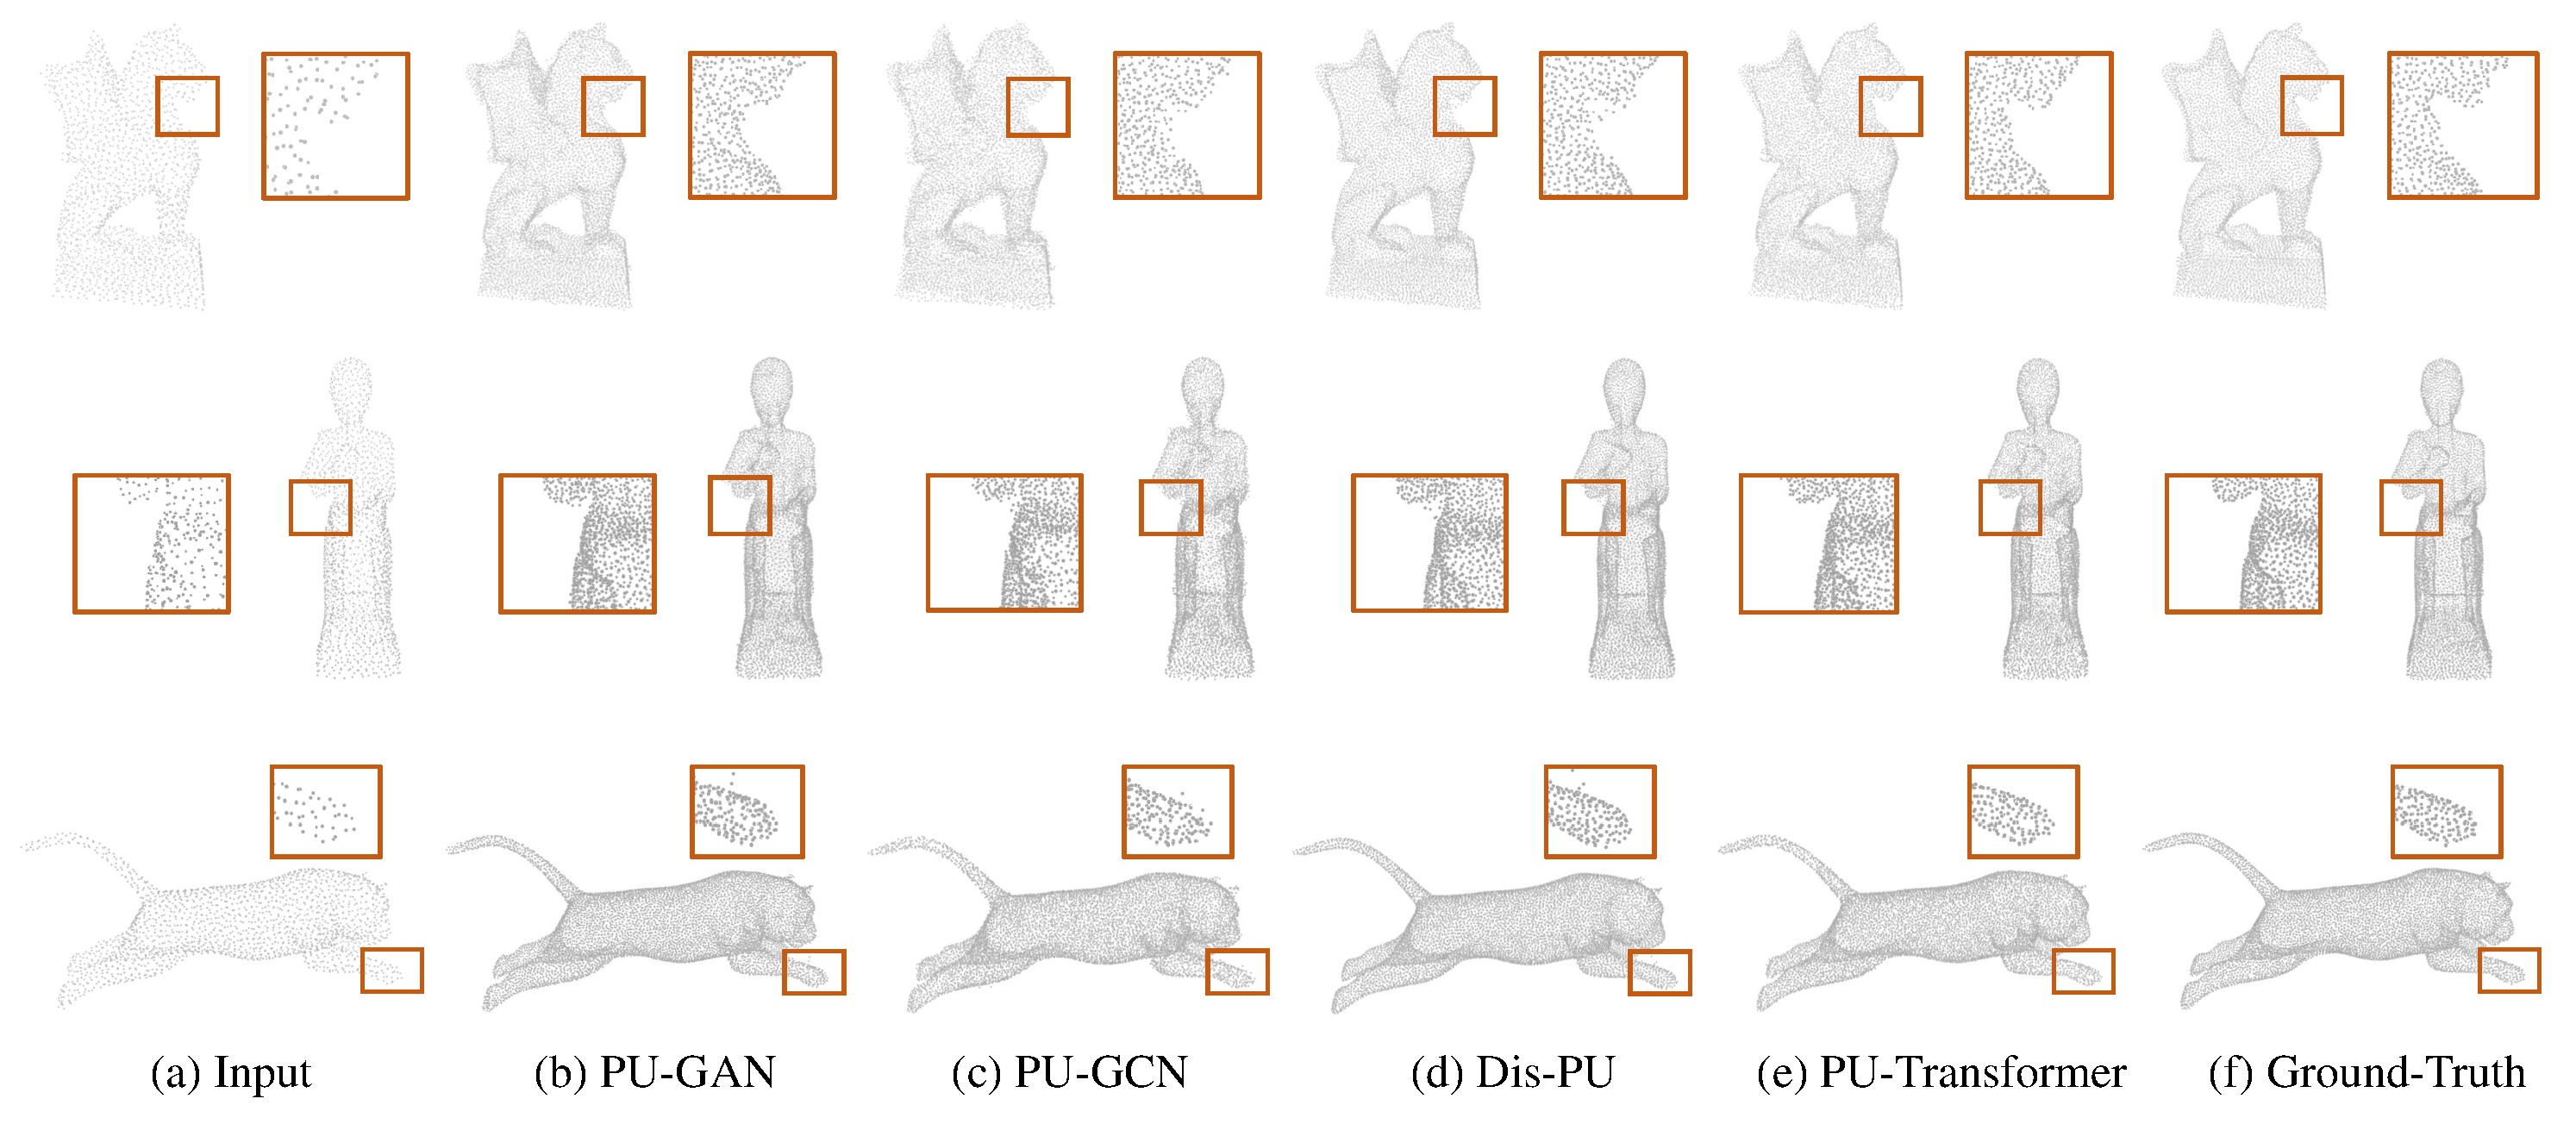
\includegraphics[width=0.98\textwidth]{images/vis_new.pdf}
\end{center}
\captionsetup{font=small}
\caption{Comparisons to state-of-the-art methods (PU-GAN~\cite{li2019pu}, PU-GCN~\cite{qian2021pu}, Dis-PU~\cite{li2021point}) in ($4\times$) upsampling \emph{synthetic} point cloud data using 2048 input points.}
\label{fig:vis}
\end{figure}

\begin{figure}[t]
\begin{center}
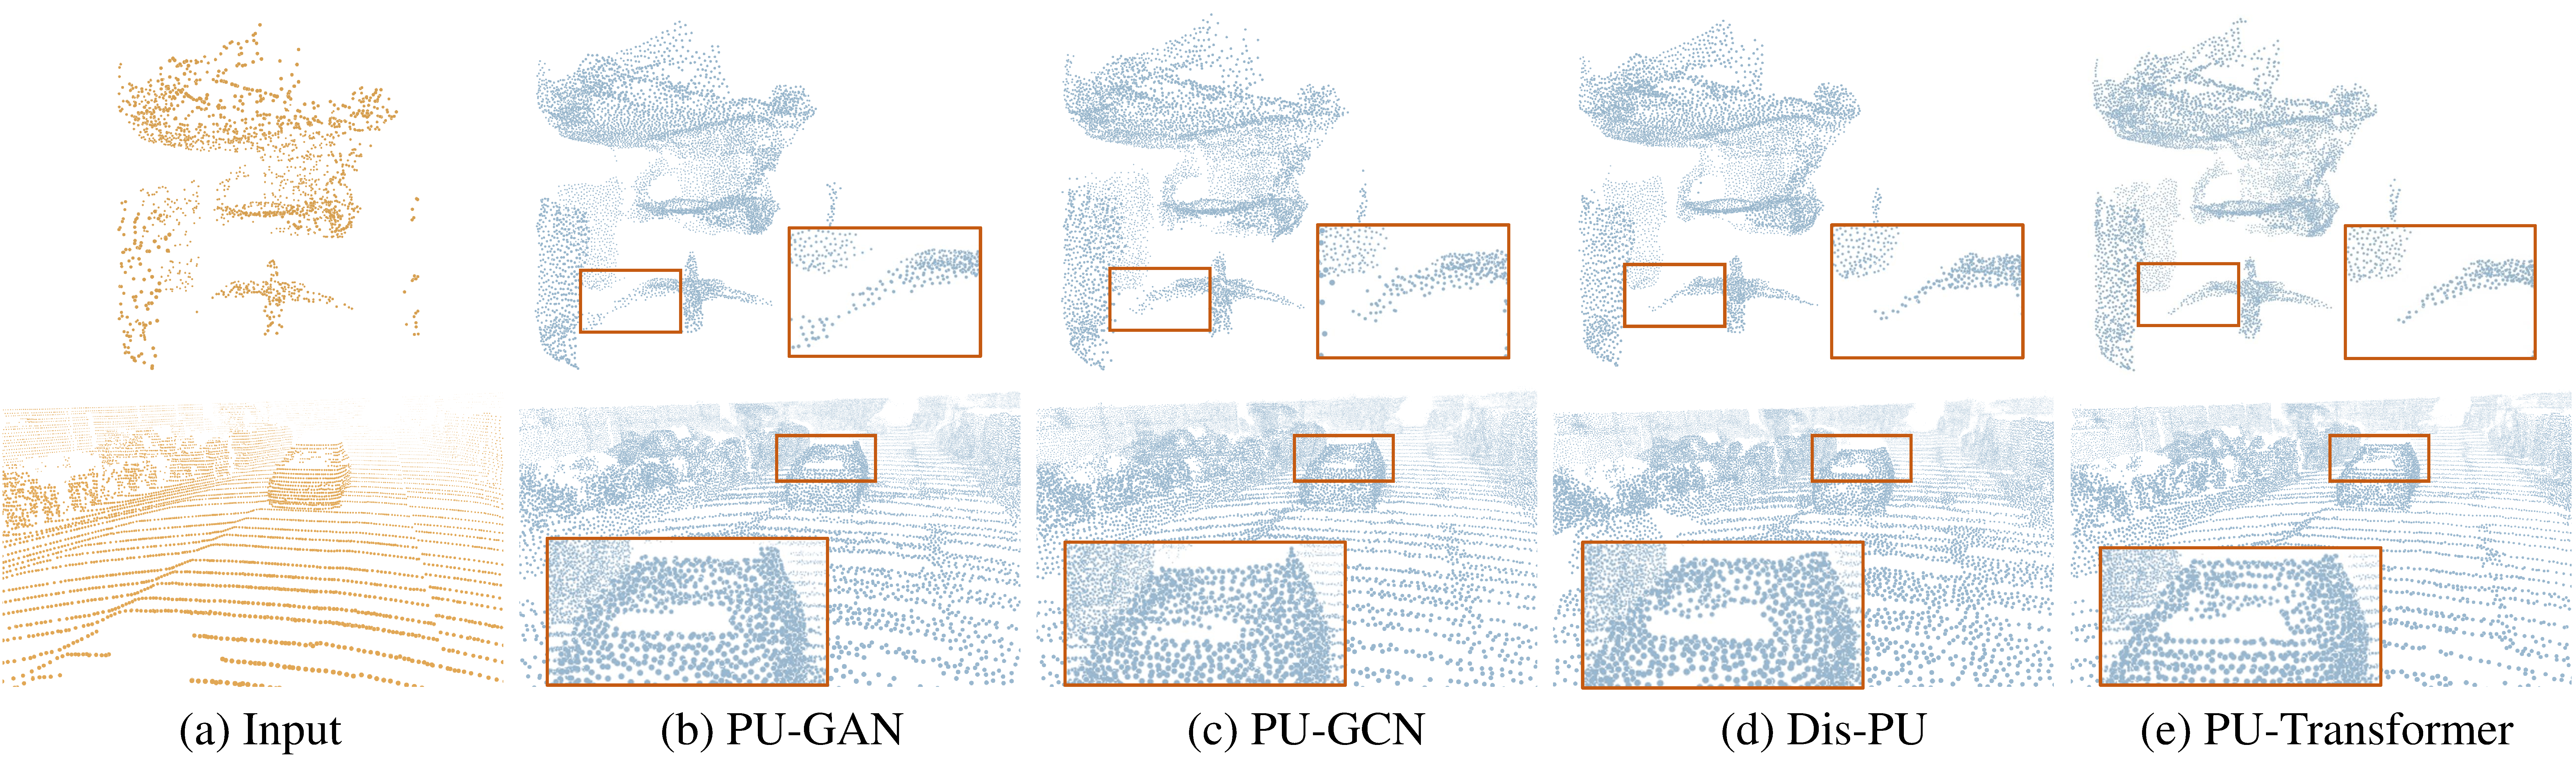
\includegraphics[width=\textwidth]{images/real_vis_new.pdf}
\end{center}
\captionsetup{font=small}
\caption{Comparisons to state-of-the-art methods (PU-GAN~\cite{li2019pu}, PU-GCN~\cite{qian2021pu}, Dis-PU~\cite{li2021point}) in ($4\times$) upsampling \emph{real} point cloud data from ScanObjectNN~\cite{uy2019revisiting} dataset and SemanticKITTI~\cite{behley2019semantickitti} dataset.}
\label{fig:vis_scan}
\end{figure}

\subsection{Visualization}
\noindent \textbf{Qualitative Comparisons:}
The qualitative results of different point cloud upsampling models are presented in Fig.~\ref{fig:vis} and~\ref{fig:vis_scan}. Since we utilize the self-attention based structure to capture the point-wise dependencies from a global perspective, the PU-Transformer's output can better illustrate the overall contours of input point clouds producing fewer outliers (as shown in the zoom-in views of Fig.~\ref{fig:vis}). Particularly, based on the rich local context encoded by our Positional Fusion block, the PU-Transformer precisely upsamples the real point clouds (compared in Fig.~\ref{fig:vis_scan}), retaining a uniform distribution and much structural detail.

\noindent \textbf{Upsampling Different Input Sizes:}
Fig.~\ref{fig:res} shows the results of upsampling different sizes of point cloud data using PU-Transformer. Given a relatively low-resolution point cloud (\eg, 256 or 512 input points), our proposed model is still able to generate dense output with high-fidelity context (\eg, the head/foot of \enquote{Panda}). As the input size increases, the new points are uniformly distributed, covering the main flat areas (\eg, the body of \enquote{Panda}). 

\noindent \textbf{Upsampling Real Point Clouds:} In addition to Fig.~\ref{fig:vis_scan}, we provide more upsampling results ($4\times$ and $16\times$) on real point cloud samples (\ie, \enquote{chair}, \enquote{office}, \enquote{room}, \enquote{street}) from \emph{ScanObjectNN}~\cite{uy2019revisiting}, \emph{S3DIS}~\cite{armeni2017joint}, \emph{ScanNet}~\cite{dai2017scannet}, and \emph{SemanticKITTI}~\cite{behley2019semantickitti}, respectively. As Fig.~\ref{fig:scan} clearly illustrates, by addressing the sparsity and non-uniformity of raw inputs, not only is the overall quality of point clouds significantly improved, but also the representative features of object instances are enhanced. Particularly, the contours of upsampled object instances (\eg, \emph{tables} in \enquote{office/room}, \emph{cars} in \enquote{street}) are clearly distinct from the complex surroundings, obtaining high-fidelity details for visual analysis. More examples for visualization are included in the supplementary material.

\noindent
\begin{minipage}[t]{0.47\textwidth}
  \vspace{0pt}
  \centering
    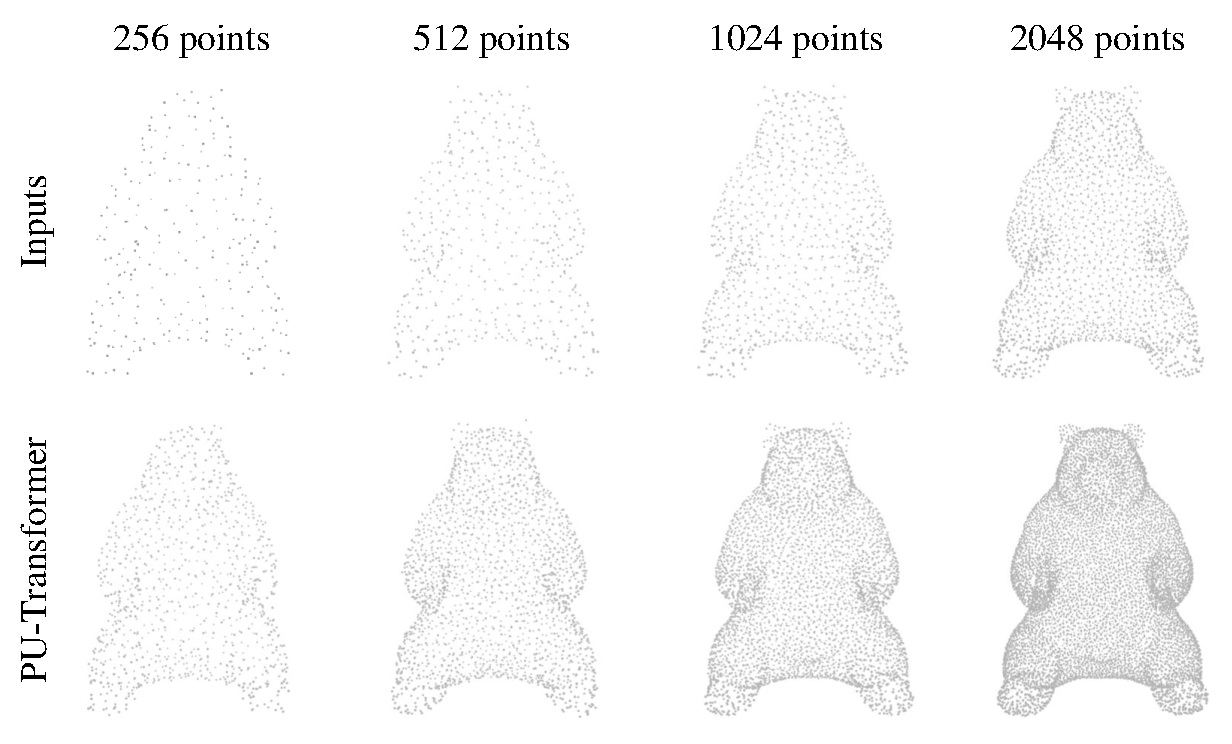
\includegraphics[width=\columnwidth]{images/res.pdf}
    \captionof{figure}{\small PU-Transformer's $4\times$ upsampling results, given different sizes of input point cloud data.}
    \label{fig:res}
\end{minipage}%
\hfill%
\begin{minipage}[t]{0.47\textwidth}
  \vspace{0pt}
  \centering
    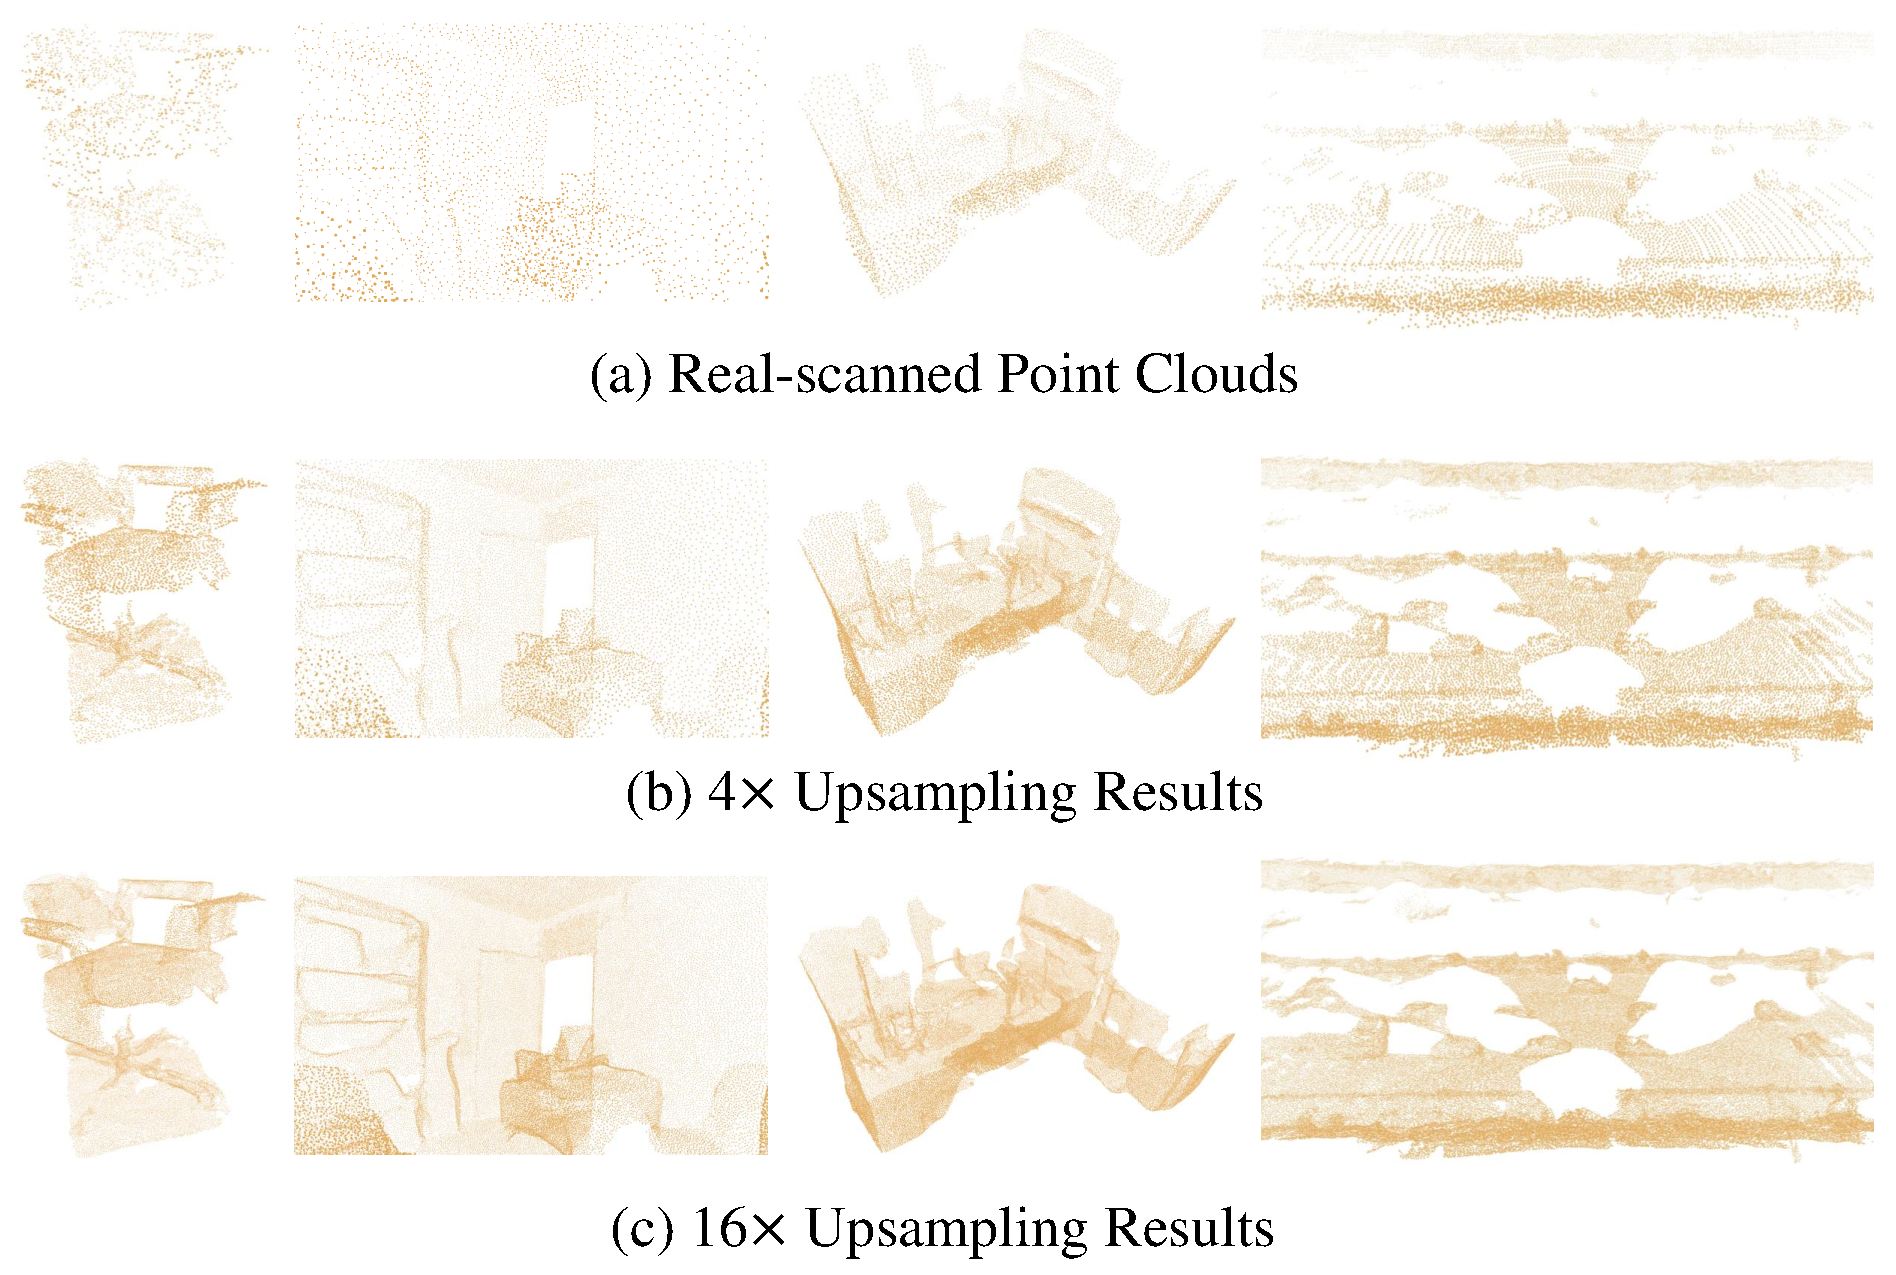
\includegraphics[width=0.9\columnwidth]{images/vis_front.pdf}
    \captionof{figure}{\small PU-Transformer's $4\times$ and $16\times$ upsampling results, given different real point clouds.}
    \label{fig:scan}
\end{minipage}